
\documentclass[11pt,compress,t,notes=noshow]{beamer}

\usepackage[english]{babel}
\usepackage{dsfont}
\newcommand\bmmax{2}
\usepackage{bm}
\usepackage{bbm}
\usepackage{verbatim}
\usepackage{amsmath}
\usepackage{amsfonts}
\usepackage{csquotes}
\usepackage{multirow}
\usepackage{longtable}
\usepackage{enumerate}
\usepackage[absolute,overlay]{textpos}
\usepackage{psfrag}
\usepackage{algorithm}
\usepackage{algorithmicx}
\usepackage{algpseudocode}
\usepackage{eqnarray}
\usepackage{multimedia}
\usepackage{media9}
\usepackage{arydshln}
\usepackage{tabularx}
\usepackage{placeins}
\usepackage{tikz}
\usepackage{setspace}
\usepackage{wrapfig}
\usepackage{tcolorbox}
\usepackage[export]{adjustbox}
\usepackage{siunitx}
\usetikzlibrary{shapes,arrows,automata,positioning,calc}
\tikzset{
  %Define standard arrow tip
  >=stealth',
  %Define style for boxes
  punkt/.style={
    rectangle,
    rounded corners,
    draw=black, very thick,
    text width=6.5em,
    minimum height=2em,
    text centered},
  % Define arrow style
  pil/.style={
    ->,
    thick,
    shorten <=2pt,
    shorten >=2pt,}
}
\usepackage{subfig}

%new environments

\newenvironment{vbframe}  %frame with breaks and verbatim
{
 \begin{frame}[containsverbatim,allowframebreaks]
}
{
\end{frame}
}

\newenvironment{vframe}  %frame with verbatim without breaks (to avoid numbering one slided frames)
{
 \begin{frame}[containsverbatim]
}
{
\end{frame}
}

\newenvironment{blocki}[1]   % itemize block
{
 \begin{block}{#1}\begin{itemize}
}
{
\end{itemize}\end{block}
}

\newenvironment{fragileframe}[2]{  %fragile frame with framebreaks
\begin{frame}[allowframebreaks, fragile, environment = fragileframe]
\frametitle{#1}
#2}
{\end{frame}}


\newcommand{\myframe}[2]{  %short for frame with framebreaks
\begin{frame}[allowframebreaks]
\frametitle{#1}
#2
\end{frame}}

\newcommand{\remark}[1]{
  \textbf{Remark:} #1
}

%%%%%%%%%%%%%%%%%%%%%%%%%%%%%%%%%%%%%%%%%%%%%%%%%%%%%%%%%%%%%%%%%%%%%%%%%%%%%%%

% basic latex stuff
\newcommand{\pkg}[1]{{\fontseries{b}\selectfont #1}} %fontstyle for R packages
\newcommand{\lz}{\vspace{0.5cm}} %vertical space
\newcommand{\dlz}{\vspace{1cm}} %double vertical space
\newcommand{\oneliner}[1] % Oneliner for important statements
{\begin{block}{}\begin{center}\begin{Large}#1\end{Large}\end{center}\end{block}}


%\usetheme{lmu-lecture}
\usepackage{../style/lmu-lecture}

\let\code=\texttt
\let\proglang=\textsf

\setkeys{Gin}{width=0.9\textwidth}


\title{Deep Learning}
\author{Mina Rezaei}
\institute{Department of Statistics -- LMU Munich}
\date{Winter Semester 2021}

\setbeamertemplate{frametitle}{\expandafter\uppercase\expandafter\insertframetitle}

%\begin{document}
%\sloppy
%\end{document}

 
\input{../../latex-math/basic-math}
\input{../../latex-math/basic-ml}
\input{../../latex-math/ml-nn}

\begin{document}
    
\lecturechapter{10}{Maximum Likelihood Estimation}
\lecture{Deeplearning}

\begin{frame}
\frametitle{Lecture outline}
\tableofcontents
\end{frame}


\section{Maximum Likelihood}

\frame{
    \frametitle{Maximum Likelihood}
    \only<1>{
        \begin{figure}
        \includegraphics[width=5cm]{plots/sample.png}
        %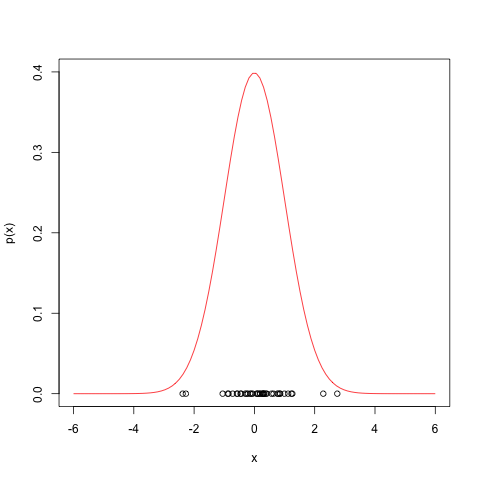
\includegraphics[width=6cm]{sample-withGaussian.png}
        \end{figure}
    }
    %\vspace{-1cm}
    \only<2-3>{
        \begin{figure}
        %\includegraphics[width=5cm]{sample.png}
        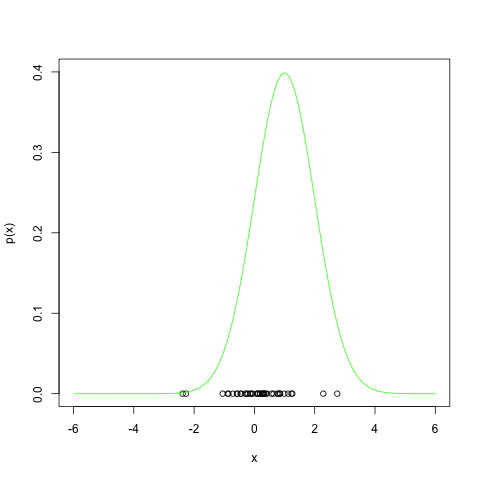
\includegraphics[width=5cm]{plots/sample-whichGaussian1.png}
        \end{figure}
    }
    \only<4>{
        \begin{figure}
        %\includegraphics[width=5cm]{sample.png}
        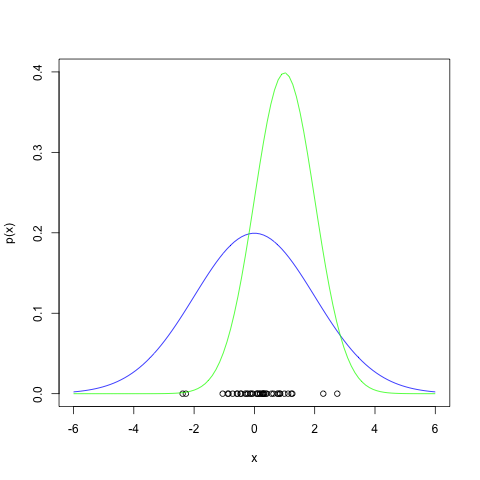
\includegraphics[width=5cm]{plots/sample-whichGaussian2.png}
        \end{figure}
    }
    \only<5>{
        \begin{figure}
        %\includegraphics[width=5cm]{sample.png}
        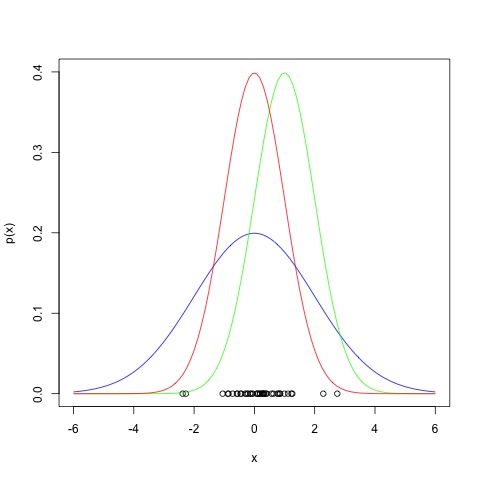
\includegraphics[width=5cm]{plots/sample-whichGaussian3.png}
        \end{figure}
    }
    %\vspace{-1cm}
    
    %We assume that the data-underlying distribution is Gaussian, that is we use a model
    We choose the model distribution $p_{\theta}$ to be Gaussian, that is
    \only<1>{
    \begin{footnotesize}
        $$p_{\thetab}(\xi)= \frac{1}{\sqrt{2\pi\sigma^2}} \exp\left(-\frac{1}{2} \frac{\left(\xi - \mu\right)^2}{\sigma^2}\right)$$
    \end{footnotesize}
    }
    \only<2-5>{
        $$p_{\thetab}\left(\xi[1],\dots, \xi[n]\right)
        = \prod_{i=1}^{n} p_{\thetab}\left(\xi\right)
        = \prod_{i=1}^{n}  \frac{1}{\sqrt{2\pi\sigma^2}} \exp\left(-\frac{1}{2} \frac{(\xi-\mu)^2}{\sigma^2}\right)$$
    }
    %\only<3-6>{
        %$$p_{\thetab}(x_1,\dots, x_n)
        %= \prod_{i=1}^{n} p_{\thetab}(x_i)
        %=  \left(\frac{1}{\sqrt{2\pi\sigma^2}}\right)^n \exp\left(\sum_{i=1}^{n} -\frac{1}{2} \frac{(x_i-\mu)^2}{\sigma^2}\right)$$
            %}
    
    \only<3-5>{
        Given $\left\{\xi[1], \dots, \xi[n]\right\}$, how should we estimate $\thetab =\{\mu, \sigma^2\}$?
    }
}

\frame{
    \frametitle{Recall: Maximum Likelihood Estimation}
    
    
    The \textbf{likelihood function} is given by
    
    $$L\left(\thetab | \xi[1],\dots, \xi[n]\right)= \prod_{i=1}^{n} p_{\thetab}\left(\xi\right)
    %=  \left(\frac{1}{\sqrt{2\pi\sigma^2}}\right)^n \exp\left(\sum_{i=1}^{n} -\frac{1}{2} \frac{(\xi-\mu)^2}{\sigma^2}\right)
    =\prod_{i=1}^{n}  \frac{1}{\sqrt{2\pi\sigma^2}} \exp\left(-\frac{1}{2} \frac{(\xi-\mu)^2}{\sigma^2}\right) \enspace.
    $$
        
        To maximize it, we  often consider the  \textbf{log-likelihood}
    
    \begin{align*}
    %l (\thetab | \xi[1],\dots, \xi[n])&=
        \log L(\thetab | \xi[1],\dots, \xi[n]) &= \log \prod_{i=1}^{n} p_{\thetab}(\xi)
    %=  \left(\frac{1}{\sqrt{2\pi\sigma^2}}\right)^n \exp\left(\sum_{i=1}^{n} -\frac{1}{2} \frac{(\xi-\mu)^2}{\sigma^2}\right)
    = \sum_{i=1}^{n} \log p_{\thetab}(\xi) \\
    &=  \log \left( \frac{1}{\sqrt{2\pi\sigma^2}} \right) -\frac{1}{2}  \sum_{i=1}^{n} \frac{(\xi-\mu)^2}{\sigma^2}\enspace.
    \end{align*}
}


\begin{frame}{Recall: Maximum Likelihood Estimation}
    
    Setting derivatives equal to zero yields
    $$
        \frac{\partial \log L\left(\thetab | \xi[1],\dots, \xi[n]\right) }{\partial \mu} = \frac{1}{\sigma^2  } \left( \sum_{i=1}^n \xi -n \mu \right)
    $$
        and
    $$
        \frac{\partial \log L(\thetab | \xi[1],\dots, \xi[n]) }{\partial \sigma} = \frac{1}{2\sigma^2  } \left(  \frac{1}{\sigma^2  } \sum_{i=1}^n (\xi -\mu)^2 -n \right)  \enspace.
    $$
        Leading to
    $$
        \hat \mu = \frac{1}{n} \sum_{i=1}^n \xi    \text{\;\;\;\;and\;\;\;\;}  \hat \sigma = \frac{1}{n} \sum_{i=1}^n (\xi- \hat \mu)^2  \enspace.
    $$
\end{frame}

\begin{frame}{Notes on maximum likelihood learning}

 \begin{itemize}\itemsep2ex
 \item For a  model $p$ with visible variables $\vec x$ and
 hidden variables $\vec z$, the likelihood computation involves
 \[
     p(\vec \xi\,|\,\vec\theta) = \sum_{\vec z} p(\vec \xi,\vec z\,|\,\vec\theta)\enspace.
     \]
 This is difficult, especially because of the sum which prevents the logarithm to
 act directly on  the joint distribution. \pause
 \item If we  can not find the maximum likelihood parameters analytically (i.e.~by setting the derivative to zero) one can  maximize the likelihood via SGD or related algorithms.
 \item If $p_{\text{data}}$ is the true distribution underlying $S$, maximizing the
 logarithmic likelihood function corresponds to minimizing an
 empirical estimate of the Kullback-Leibler divergence
 $KL(p_{\text{data}}\,\|\,p)$.
 \end{itemize}
 \end{frame}

%\begin{vbframe}
%\frametitle{Kullback-Leibler divergence}
%Kullback-Leibler (KL) divergence between two distribution $p$ and $p_{\text{data}}$
%over $\vec x$  is
%\smallskip
%\begin{itemize}%\normalsize\itemsep2ex
%\item a (non-symmetric) measure of
%  difference between
%% distributions,
%$p$ and $p_{\text{data}}$,
%\item always positive, zero iff the distributions are the same,
%\end{itemize}\pause
%and defined as
%\begin{align*}
%\KL(p_{\text{data}}\,\|\,p)
%&= -\sum_{\vec x} p_{\text{data}}(\vec
%x)\ln\frac{p(\vec x)}{p_{\text{data}}(\vec x)} \\
% &= -\fub{\sum_{\vec x} p_{\text{data}}(\vec
%x)\ln p(\vec x)}{can be approximated by $\frac{1}{\ell}\sum_{n=1}^{\ell} \ln p(\xb_n)$}  +\fub{\sum_{\vec x} p_{\text{data}}(\vec
%x)\ln      {p_{\text{data}}(\vec x)}}{{independent of $p$}}
%\end{align*}
% (sum turns to integral for
%  continuous random variables).
%\end{vbfram%e}




\endlecture
\end{document}
